\subsection{Dimer}
\label{sec:dimer}

The Dimer algorithm~\cite{dimer-original-1999} is in essence a method for finding the eigenmode corresponding to the lowest eigenvalue of the Hessian, while performing no direct calculations of the second derivatives.
This information is then used to locate \sap1s.

Given only an initial point, $\vR$, on a multidimensional function, $V(\vR)$, the goal is to, iteratively, locate a nearby \sap1, using no direct calculation of the Hessian, i.e. using only the function's values and its gradient, $\nabla V(\vR)$.
Indirect information about the Hessian is, however, used in the form of an estimate of the eigenmode corresponding to its lowest eigenvalue (the minimum mode).
Using the minimum mode, $\uvn$, it is possible to locally transform \sap1s to minima while using conventional techniques to move up-hill and locate the \sap1.

The dimer method can be split into three independent phases.
\ben{dimer-phases}
\item Estimating the minimum mode.
\item Transforming the gradient to make \sap1 seem as minima.
\item Translating the point according to the transformed gradient.
\een
Only the first of the phases is unique to the dimer algorithm.
A setup phase, which typically includes randomly displacing $\vR$ is also required if the search starts from a minimum.

\subsubsection{Minimum Mode Estimate}
\begin{figure}[t]
  \begin{center}
    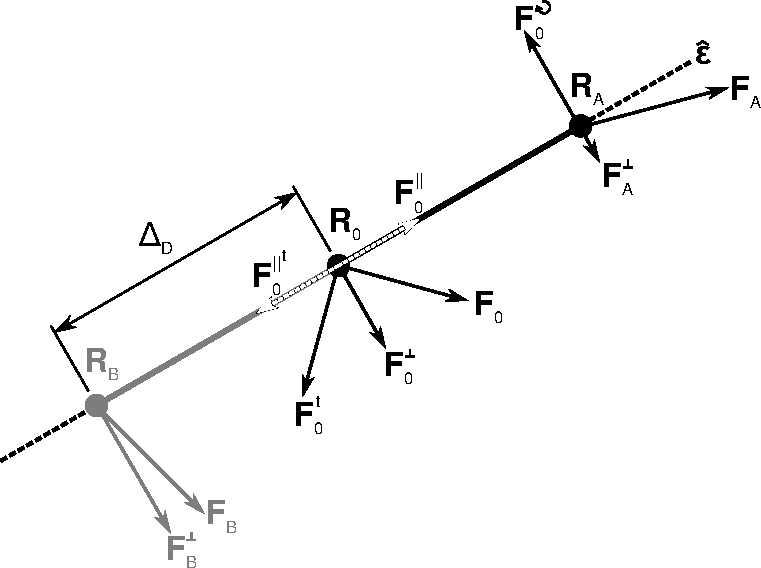
\includegraphics[width=0.6\linewidth]{dimer-force-overview}
\parbox{0.85\linewidth}{\caption{A schematic overview of the force components acting within the dimer method.
$\vR_\text{A}$ and $\vR_0$ are the positions of the dimer images with the greyed out $\vR_\text{B}$ as the virtual image (\fref{eq:dimer-point-extrapolate}).
Each force component is labeled with super- and subscripts as follow:
$0$, $\text{A}$ and $\text{B}$ in subscripts refer to at which point they are calculated,
$\perp$ and $\parallel$ in superscripts refer to the specific component of the full force (perpendicular and parallel to the minimum mode estimate, respectively),
$\text{t}$ in a superscript refers to the transformed force (\fref{eq:dimer-transform}),
$\circlearrowright$ refers to the rotational force (\fref{eq:rotational-force}) and no superscript refers to the PES force.
$\Dsep$ is the distance between dimer points (\fref{eq:dimer-separation} and $\uvn$ is the current minimum mode estimate.
\tblue{There is no reference to this figure in the text.}
}
\label{fig:dimer-force-overview}
}
  \end{center}
\end{figure}

\tblue{Inspired by the hyperdynamics method by Voter~\cite{hyperdynamics-voter-1997}.}

Estimating the second derivative of $V$ along a given unit vector, $\uvs$, at point $\vR$ can be done numerically, using finite differences.
For the occasion, a pair of points (the dimer), $[\vR_\text{A}, \vR_\text{B}]$, are chosen, close to current point $\vR_0$, such that
\beq{dimer-separation}
\vR_\text{A} = \vR_0 + \Dsep \uvs \quad \text{and} \quad \vR_\text{B} = \vR_0  - \Dsep \uvs,
\eeq
where $\Dsep$ is a predefined constant to determine the length of the dimer and the separation in the finite difference estimate.
Using only the function's values, the second derivative (or curvature), $C_\vs$, becomes
\beq{second-derivative-function}
C_\vs \equiv \frac{\partial^2 V}{\partial \uvs^2} \approx \frac{V_\text{A} + V_\text{B} - 2V_0}{\Dsep^2},
\eeq
where $V_\text{x} \equiv V(\vR_\text{x})$.
As the gradient points away from each minimum, it is convenient to define a force, $\vF$ that points towards minima instead, for use in the iterative minima search,
\beq{gradient-force}
\vF_\text{x} \equiv - \nabla V(\vR_\text{x}).
\eeq
Should the gradient is readily available, as it often is, \fref{eq:second-derivative-function} can be rewritten to depend on it instead,
\beq{second-derviative-gradient}
C_\vs \approx \frac{(\vF_\text{B} - \vF_\text{A}) \cdot \uvs}{\Dsep}.
\eeq
Rotating $\uvs$ around $\vR_0$, according to the rotational force,
\beq{rotational-force}
%\vF^\circlearrowright = (\vF_\text{A} - (\vF_\text{A} \cdot \uvs)\uvs) - (\vF_\text{B} - (\vF_\text{B} \cdot \uvs)\uvs)
\vF^\circlearrowright = \vF_\text{A} - \vF_\text{B} + ((\vF_\text{B} - \vF_\text{A}) \cdot \uvs)\uvs,
\eeq
until $C_\vs$ is minimized yields an estimate for, both, the lowest eigenvalue, $C_\text{min} = C_\vs$, of the Hessian and its corresponding eigenmode, the minimum mode, $\uvn$.
The rotation happens in a plane spanned by $\uvn$ and $\uvT \equiv \vF̣^\circlearrowright / \left| \vF^\circlearrowright \right|$
A number of rotational schemes can be employed, such as a finite difference, conjugate gradient, approximation~\cite{dimer-original-1999} and, as described in~\cite{dimer-heyden-2005}, by expanding the curvature, exactly, as a Fourier series.
Both of the mentioned schemes require extra calculations to figure out the optimal angle of rotation but the latter is better suited when the accuracy and/or consistency of the force cannot be guaranteed~\cite{dimer-heyden-2005}, e.g. when doing DFT calculations.

Often $\vF_0$ is calculated to get a more accurate translational force, this can be taken advantage of in order to cut down the amount of computations.
Assuming a quadratic behaviour near the dimer, the gradient at either of the dimer's endpoints can be extrapolated from the other endpoint and the central point~\cite{dimer-olsen-2004},
\beq{dimer-point-extrapolate}
\vF_\text{B} = 2\vF_0 - \vF_\text{A},
\eeq
with $\vF_\text{B}$ being the extrapolated, virtual, force.
Since $\vF_0$ is static and does not require additional calculations during the iterative rotation, performing this extrapolation yields significant calculational reductions, up to a factor of half.

Further extrapolations are possible, if multiple rotations are performed (which is often not the case), it is possible to use previous calculations of either end point to extrapolate the rotated values.
These, however, yield much less reductions than the extrapolation in \fref{eq:dimer-point-extrapolate}.

\subsubsection{Gradient Transformation}
Once a minimum mode estimate is available for the current point, $\vR_0$, it is possible to transform the force so that any \sap1 is transformed to a minimum.
As discussed above, \sap{1}s are stationary (with zero gradient) and the Hessian has one and only one negative eigenvalue.
The goal is thus to maximize the function's value along the minimum mode while minimizing it along all other eigenmodes.
This can be achieved, simply, by inverting any force components along the minimum mode,
\beq{dimer-transform}
\vF_0^\text{t} = \vF_0 - 2(\vF_0 \cdot \uvn)\uvn.
\eeq
In cases were the dimer aligns itself with a contour of the potential in a convex region (where the Hessian has only positive eigenvalues), it is possible that a lot of time will be spent there.
In order to circumvent this, a different force transformation,
\beq{dimer-transform-minima}
\vF_0^\text{t} = -(\vF_0 \cdot \uvn)\uvn ,
\eeq
is often used in convex regions.
This latter transformation simply inverts the force along the minimum mode while ignoring any other components.
This along with a fixed, artificially large, step size should yield less iterations spent near minima and more near \sap1s.~\cite{dimer-original-1999}

\subsubsection{Iterative Translation}
After the force has been transformed such that \sap1s appear as minima - \sap1s, however, remain unchanged with regards to the function's value - it is possible to use conventional algorithms for finding minima as long as they support a systematic increase in the function's value.
A finitie difference method was suggested in the original implementation~\cite{dimer-original-1999} while more recent papers~\cite{dimer-kastner-2008} have used other methods, such as the L-BFGS algorithm~\cite{lbfgs}.
